\documentclass{mcmthesis}
\mcmsetup{CTeX = false,   % 使用 CTeX 套装时,设置为 true
        tcn = 55869, problem =  C,
        sheet = true, titleinsheet = true, keywordsinsheet = true,
        titlepage = false, abstract = true}
\problem{C}

\makeatletter % `@' now normal "letter"   %follpw as section test
\@addtoreset{equation}{section}
\makeatother  % `@' is restored as "non-letter"
\renewcommand\theequation{\oldstylenums{\thesection}%
                   .\oldstylenums{\arabic{equation}}}
\newcommand{\upcite}[1]{\textsuperscript{\textsuperscript{\cite{#1}}}}
\usepackage{palatino}
\usepackage{mwe}
\usepackage{graphicx}
\usepackage{tabularx}
\usepackage{float}
\usepackage{indentfirst}
\usepackage{amsmath}
\usepackage{caption}
\usepackage{subfigure}
\usepackage{makecell}
\title{}
\date{}

\begin{document}

\begin{abstract}%摘要


\title{Keep the Bathtub Warm}



\end{abstract}

\begin{keywords}
	\textbf{A,\indent B, \indent}
\end{keywords}
\maketitle
\tableofcontents\thispagestyle{empty}
%设置页眉
\newpage

\setcounter{page}{1}
%Section 1
\section{Introduction}
\subsection{Literature review}
\indent Traffic flow modeling as the basis of traffic control, traffic design, traffic analysis, traffic simulation and traffic control decision making always is the the research focus in traffic engineering field. And it can be divided into macroscopic and microscopic models from the angle of study, mainly using the theory of fluid mechanics and the theory of car following\upcite{TF1}. Due to their accuracy and practicability, these two models play an important role in the development of traffic flow modeling\upcite{TF2}.\\
\indent The cellular automata (CA) is a kind of grid dynamical model in which time, space and state are discrete, and the space interaction and time causality are local. It has the ability to simulate the spatio-temporal evolution process of complex systems. The study of single lane traffic flow cellular automaton model began in 1986, the most famous of them is the NS model proposed by Nagel and Schreeckenberg in 1992\upcite{ca1}. However, this model has a great flaw, and has been gradually improved by follow-up scientists. Such as the T2 model\upcite{ca2} put forward by Takayasu and the VDR model\upcite{ca3} put forward by barlovic. Cellular automata is now always used to calculate traffic flow problems.\\


\section{Assumptions}
\noindent
{\bf (1) } \textbf{example.} example.\\

\section{Symbols}
\begin{table}[H]
        \setlength{\abovecaptionskip}{0pt}
        \setlength{\belowcaptionskip}{0pt}
				\centering{Table 1:Constants}\\
        \begin{tabular}{p{2cm}|p{2cm}|p{7.5cm}|p{1.7cm}}
		\hline
		\rowcolor[gray]{0.9}\bf{Symbol}	&\bf{uint}      &\bf{Meaning}&\bf{value}	\\
		\hline
		${P}''_{v}$		& $hP_{a}$		 & example  &12\\

		\hline
	\end{tabular}
\end{table}

\begin{table}[H]
        \setlength{\abovecaptionskip}{0pt}
        \setlength{\belowcaptionskip}{0pt}
        \centering{Table 2:Notation} \\
        \begin{tabular}{p{1.8cm}|p{2.2cm}|p{9cm}}
        \hline
        \rowcolor[gray]{0.9}\bf{Symbol}	&\bf{uint}      &\bf{Meaning}\\
        \hline
        $C_{i}$	&$ $ &the $i$ th vehicle\\
        $t_{i}$	&$ $ &the Time Headway between $ C_{i} $ and the front vehicle\\
        $T$	&$s$ &the average Time Headway in a road\\
        $F(t_{i})$	&$ $ &the distribution function of $t_{i}$
\\
        
        \end{tabular}
        \end{table}

\section{Models}
\subsection{Data preprocessing}
Data preprocessing is mainly to extract the data from the Excel and calculate the traffic flow of a single lane. And the daily traffic flow in each lane is\\
\begin{equation}
N=Counts/(Decr+Incr)
\end{equation}

where $Counts$ is Average daily traffic counts Year\_2015, $Decr$ is the Number of Lanes DECR MP direction and $Incr$ is the Number of Lanes Incr MP direction. And the influence of the number of lanes will be discussed in \ref{lanes}.\\


\subsection{Design of Cellular Automata }
Large quantities of former traffic simulations based on Cellular Automata (CA) indicate that CA model is a feasible and effective method to emulate traffic flow. Space, time and status are all discrete in Cellular Automata. \\
\indent For example, The model abstracts the car into a particle, and time is divided into small units. This feature predigests the simulation process significantly. Besides, the status of a cell is controlled by its neighboring cells following a set of rules, which is much similar to real-life traffic where a car's movement largely depends on its neighboring cars' movements. Therefore, it is rational for us to apply Cellular Automata in solving our problem.\\
\subsubsection{The data structure of cellular automata}
We set 5 attributes for each car, including the position ($p$), the distance from the front car ($d$), the speed ($v$), the driver's head time ($t$), the type of the car ($k$).\\
\indent The property vector of each car can be expressed as
\begin{equation}
	car_{i}=\left [ p_{i},d_{i},v_{i},t_{i},k_{i} \right ]
\end{equation}
\indent The properties of all the cars can be superimposed and combined into a two-dimensional matrix, the matrix is as follows
\begin{equation}
	Cars=
	\begin{bmatrix}
	   car_{1}\\
	   car_{2}\\ 
	   ...\\ 
	   car_{n}
	\end{bmatrix}
	=
	\begin{bmatrix}
		p_{1},d_{1},v_{1},t_{1},k_{1}\\
		p_{2},d_{2},v_{2},t_{2},k_{2}\\ 
		...\\ 
		p_{n},d_{n},v_{n},t_{n},k_{n}
	\end{bmatrix}
	=
	\left [ P,D,V,T,K \right ]
\end{equation}
where $P, D, V, T, K$ are column vectors. For example\\
\begin{equation}
V=\left [ v_{1},v_{2},...,v_{n-1},v_{n} \right ]^{T}
\end{equation}
\indent $P$ is a column vector for all vehicle locations, which unit is kilometer. $D$ is the distance between each car and the previous one. $D$ can be calculated as follows
\begin{equation}
D=[P^{T}(2:n)-P^{T}(1:n-1),0]^{T}
\end{equation}
$V$ is a column vector for all vehicle speed, which unit is km/h. The initial value of $V$ is a random vector which obeys normal distribution.  $T$ is the headway of all drivers or self-driving systems. And $K$ is all vehicles' types. The meaning and value of the headway will be given in \ref{headway}. There are two kinds of values in $k_{i}$, $0$ means self-driving car and $1$ means manual-driving car.

\subsubsection{The Integral Structure of Cellular Automata}
The model of Cellular Automata is mainly based the following aspects\\

\indent\textbf{Speed change mechanism\\}
\indent The change of speed is based on the Time Headway, the distance from the front car, the speed of the front car, and the type of the vehicle. The model will be given in \ref{velocity change}.

\indent\textbf{The calculation of position and vehicle distance\\}
\indent The calculation of position and vehicle distance is based on the speed ($V$) and the position of the last moment. The model will be given in \ref{velocity change}.

\indent\textbf{Changes in the number of cars\\}
\indent The inflow of vehicles in a section of the road consists of two parts. The first part is the inflow of the starting position of the road. The second part is the flow of cars from auxiliary road to the main road. \\
\indent The outflow of vehicles include the outflow of the end position of the road and the flow from the main road to auxiliary road.\\
\indent And the changes in the number of cars will be analyzed in the detail in \ref{changes of cars}.\\

\indent\textbf{The integral structure of single step of the simulation\\}
\indent Cellular automata simplifies the problem by discretization of the model. Figure \ref{process} shows the single step of the simulation.
\begin{figure}[H]	%图1.3
	\centerline{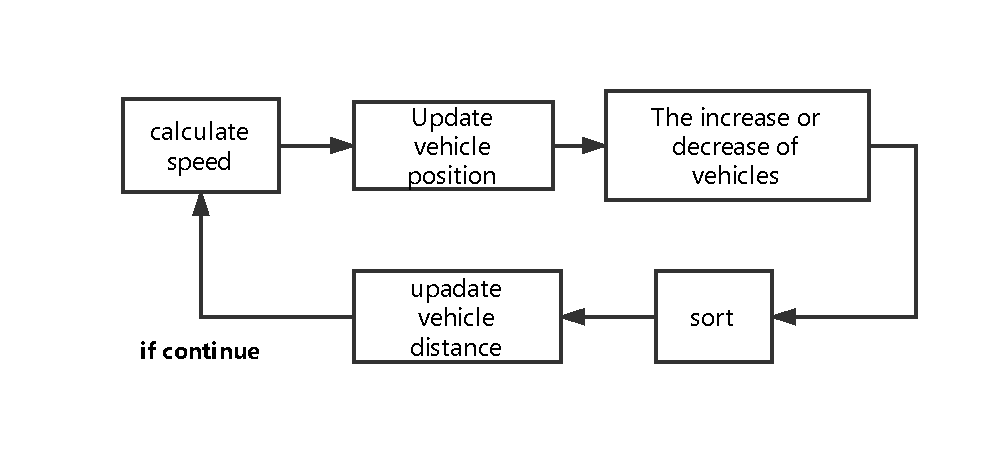
\includegraphics[height=6.5cm]{process.pdf}}
	\caption{Single step of the simulation}
	\label{process}
\end{figure}
\indent We set the step length of the simulation to be 1 second. And the simulation results are analyzed and verified in the later paper.
\subsection{Time Headway}
\label{headway}
\subsubsection{The Set of Time Headway}
\indent Time Headway (TH) is the time difference between the two adjacent vehicles passing through the same location. In general, the TH is a random value. But when people drive a car, the front car has an emergency brake or deceleration in a very short time, the following car driver can respond only after a certain reaction time. It is easy to cause traffic accidents if the distance between the two cars is two small. So the TH between the two cars needs to be greater than a minimum safety TH. The safety TH is depended on the reaction time of person.\\
\indent The TH of two vehicles is determined by the subjective judgment of the driver. But generally speaking, when the rear car is far away from the front car, the rear car will speed up and make the TH of two cars smaller. When the driver of rear is aware that the TH is too small, as the TH of reality is less than the TH he expected, the driver will slow down and increase the TH between two cars.\\
\indent Then the ratio distribution of the headway of the car needs to be determined. We can know from the previous research\upcite{TH}, when there is a minimum safety TH and crowding, the shift negative exponential distribution(SNED) can well reflect the distribution of the headway of a large number of vehicles.\\
\indent So the random variable follows the SNED model. It means,
\begin{equation}
		F(t)=1-e^{-\frac{t_{i}-\tau }{T-\tau}}
\end{equation}
\indent Where, \\
\indent $T$ is the average Time Headway in a road.\\ 
\indent In traffic flow theory, traffic flow density.\\
\begin{equation}
\begin{split}
 K = \frac{Q}{V}\\
 D_{a}=\frac{1}{K}=\frac{V}{Q}
\end{split}
\end{equation}
\indent Where, \\
\indent $K$ is the traffic flow density;\\ 
\indent $Q$ is the traffic flow;\\
\indent $V$ is the average velocity of vehicles;\\
\indent $D_{a}$ is the average distance of vehicles.\\
\indent Because the average Time Headway is the ratio of the average distance $D_{a}$ to the average velocity $V $,\\
\begin{equation}
	T=\frac{D_{a}}{V}=\frac{1}{Q}
\end{equation}
\indent It means the average distance is the reciprocal of the traffic flow.
\subsubsection{The generation of Time Headway following SNED model}
\indent When the parameters $T, \tau $ in $F(t)$ are obtained, we need to produce a large number of data that follows the SNED.\\
\indent MATLAB can only produce a group of data following the uniform distribution. To produce a group of data following $ F(t_{i})=1-e^{-\frac{t_{i}-\tau}{T-\tau}},t_{i}>\tau $, we consider a random variable, 
\begin{equation}
	t_{i}=F^{-1}(t_{i})=G(u)=\tau-(T-\tau)\cdot ln(1-u)
\end{equation}
\indent $G(u)$ is the inverse function of $F(t)$.\\
\indent When $ u \sim U(0,1) $, for some constant number $t_{0}>\tau$,\\
\begin{equation}
\begin{split}
	P\{t_{i}\leqslant t_{0}\}&=P\{\tau\leqslant t_{i} \leqslant t_{0} \}\\
&=P\{ G^{-1}(\tau)\leqslant u \leqslant G^{-1}(t_{0})\}\\
&=\int_{G^{-1}(\tau)}^{G^{-1}(t_{0})}f(u)du\\
&=\int_{F(\tau)}^{F(t_{0})}f(u)du\\
&=\int_{F(\tau)}^{F(t_{0})}1du=F(t_{0})-F(\tau)
\end{split}
\end{equation}
\indent Because the minimum Time Headway is $\tau$, $ t_{i} $must be larger than $\tau$ ,so\\
\begin{equation}
	F(\tau)=P{t_{i}<\tau}=0
\end{equation}
\begin{equation}
	P\{t_{i} \leqslant t_{0} \}=F(t_{0})
\end{equation}
\indent It means $t$ follows the SNED $F(t_{0})$.Therefore, the conclusion is obtained that when $ u \sim U(0,1) $, function type random variable follows SNED with parameters $\tau , T $. \\

\subsection{The model of calculating $P$ and $D$}
\subsubsection{Calculation of the initial $P$}
\indent $P$ is a column vector including the location of all the vehicles (the unit of $P$ is km). With the process of simulation, $P$ is a vector that varies orderly. So we only need to consider how to determine the initial value of $P$.\\
\indent In our CA model, vehicles are distributed across the whole road from the beginning of simulation. And we set the difference between every startMilepost and endMilepost as the section. From the given data sheet, we know that the traffic flow is different in different section of the road. So the distribution of vehicles is not uniform.\\
\indent At the same time, the conclusion is obtained that the length of each section of the road is about 1 to 2 kilometers, and every road has about dozens of sections. So in one section of the road, the distribution has little influence on the whole distribution of vehicles. Therefore, we suppose that in every one section of road, the distribution of the vehicles is uniform. \\
\indent From the given data sheet, we can get the start and end, The proportion of traffic flow in the peak period accounts for 8\% of the whole and $Q_{i}$ in every section of the road. By calculating, we can get the length of every section $l_{i}$ and the number of vehicles $n_{i}$ at some moment.\\
\indent We discuss the value of $n_{i}$ in two situation between the perus hour and non-peak time of the vehicle. 
\begin{equation}
	n_{i}=\begin{cases}
	&\frac{0.08Q}{3600t_{1}}\cdot\frac{l_{i}}{V_{i}} \indent\indent\indent \indent\quad\text{\,\,in the peak time }\\ 
	&\frac{0.92Q}{3600(24-t_{1})}\cdot\frac{l_{i}}{V_{i}}\indent\indent\indent \quad\text{in the non-peak time } 
	\end{cases}
\end{equation}
\indent While $v_{i}$ means the average speed of cars and $t_{i}$ is the length of the rush hour.\\
\begin{equation}
	p_i=(i-1)\cdot\frac{l_{n}}{n_{i}}+startmilepost \indent \indent	i=1,2,3,…n
\end{equation}
\indent The $p_{i}$ refers to the distance between the $i$th car and the starting point of the road.

\subsubsection{Calculation of $D$}
After we get the position vector $P$ of all vehicles, we can update the vehicle distance vector $D$. We can update all the data by the operation of the vector.The calculation method is as follows
\begin{equation}
\begin{split}
	d_i=p_{i+1}&-p_{i}\\
	D=[P(2:n)&-P(1:n-1);0]
\end{split}
\end{equation}

\subsection{The model of calculating $V$}
\label{velocity change}
\subsubsection{$\Delta V$ of Manual-driving car}
Because people want to keep their time headway as stable as possible, the first part of speed change is based on time headway. The difference between actual and expected Time Headway is
\begin{equation}
	\Delta t_{i}=t_{i}-\frac{d_{i}}{v_{i}}
\end{equation}
\indent We first directly put $\Delta t$ as the coefficient of vehicle acceleration. But we find the range of T is very large. So we use tanh function which is widely used in Neural network to normalize it.\\
\begin{figure}[H]
	\centerline{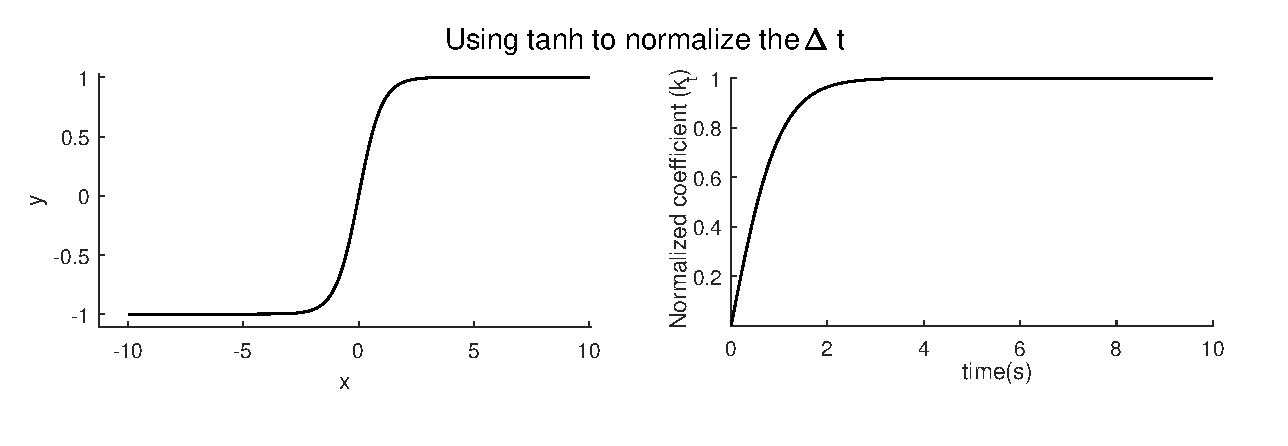
\includegraphics[height=5cm]{tanh.eps}}
	\caption{Normalization of $\Delta t_{i}$ by tanh function}
\end{figure}
\indent In the form of vector, we can get the following
\begin{equation}
\begin{split}
	\Delta T=T-D./V\\
	K_{t}= tanh(\Delta T) 
\end{split}
\end{equation}
where $t_n=0$.\\
\indent And the velocity variation $\Delta V_{1}$ caused by $\Delta T$ is
\begin{equation}
	\Delta V_{1}=K_{t}.*A
\end{equation}
\indent where A is a vector of random $a_{i}$, and $a_{i}$ is the maximum acceleration of the $i_{th}$ vehicle with uniform distribution. The unit of $a_{i}$ is $m/s^{2}$ and $a_{i}\sim U(1.1,2.1)$.\\
\indent When the speed of the rear car is higher than that of the front car, the acceleration of the rear car will be reduced to prevent pileup. The velocity variation $\Delta V_{2}$ caused by reducing acceleration in advance.
\begin{equation}
\begin{split}
	\Delta v_{2}(i)=k(v(i)-v(i+1))\\
	\Delta V_{2}=k(V-[V(2:n);0])
\end{split}
\end{equation}
where $v_2(n)=0$.\\
\\Through the experiment, we set $k$ to 0.15. And the amount of change in the speed of a single simulation step is
\begin{equation}
\Delta V=\Delta V_1-\Delta V_2
\end{equation}

\subsubsection{$\Delta V$ of Self-driving car}
The analysis of velocity variation $\Delta V_{1}$ caused by $\Delta T$ is basically the same with the Manual-driving car. But the precision of autopilot is much higher. The Time Headway of an automatic driving vehicle can be shorter than that of a man. So we can set the Time Headway of automatic to be a constant. If $k_i=0$,$t_i=2$.\\
\indent In addition to having less TH time, autopilot can have a more stable speed. We discuss the speed according to the type of car and it's front car.\\

\textbf{Cooperation between self-driving cars \\}

\textbf{Interaction between self-driving and manual-driving vehicles \\}


\subsection{Model of evaluation criteria for the degree of congestion}\
\label{evaluation criteria}
An evaluation criteria is built to evaluate the degree of congestion.\\ 
\indent When the speed distribution of all the vehicles on the road is very uniform, or even the speed of each vehicle is almost the same, the vehicles on the whole section of road needn't speed up or speed down. Each vehicle can keep the same fast speed, and because every two vehicles can be regarded as relatively stationary, there will almost be no congestion. Because the speed distribution is very uniform, the deviation between the speed and the average speed of all the vehicles is small.\\
\indent When there is a congestion on a road, the average velocity of the vehicles must be slow. When there is a congestion only in one part of the road, the velocity in this part must be much lower than the average velocity $ V_{i} $. So the speed distribution must be not uniform. Therefore, the deviation between the speed and the average speed of each vehicle is large.\\  
\indent The conclusion is obtained that the degree of congestion must be related with the average speed of the speed of all vehicles in the section of the road and the deviation between the speed and average speed of all the vehicles.\\
\indent For some section of the road, at some moment $t$, the velocity of every vehicle can be obtained. So we can use $ V_{i} $ as the first index to evaluate the degree of congestion. Therefore, the smaller $V_{i}$ of a road is, the more serious the crowding the road is.\\
\indent And we use the standard deviation of the speed of all the vehicles $S_{i}$ to evaluate the degree of congestion. However, the larger the average velocity is, the larger the absolute value of the deviation is. To represent the degree of the road more objectively, we use relative deviation $\alpha_{i} =\frac{S_{i } }{V_{i}} $ as the congestion evaluation index. The larger $\alpha w_{i}$ is, the more serious the crowding the road is.\\
Therefore, our evaluation criteria for the degree of congestion includes: $V_{i}, \alpha_{i} $. More crowding road must have a smaller $V_{i}$ and a larger $alpha_{i}$.\\
 
\subsection{The model of changes in the number of cars}
\label{changes of cars}
\subsubsection{Monte Carlo Method}
\indent Next, we consider the Monte Carlo method to simulate the change in the number the vehicle.\\
\indent Monte Carlo method is a stochastic simulation method based on probability and statistical theory. It is a method of using random numbers to solve many computational problems. In order to obtain the approximate solution of the problem, the problem is connected with a certain probability model. \\
\subsubsection{The Establishment of the Model}
\indent From the known data, we can get the traffic inflow on each road section of the day. The value of net inflow or net outflows of cars is the difference between the traffic flow of two adjacent road sections for one day.\\
\indent In the model of the cellular automata, the time to simulate one step is a second. So we should consider the net flow of cars at unit time as $\Delta n$. And the traffic conditions on the road divided into the peak hour and non peak hour. We can get
\begin{equation}
	\Delta n=\begin{cases}
	&(Q_{i}-Q_{i-1})\cdot \frac{0.08}{t_{i}\cdot 3600} \indent\indent\indent \indent\quad\text{\,\,in the peak time }\\ 
	&(Q_{i}-Q_{i-1})\cdot \frac{0.92}{(24-t_{i})\cdot 3600}\indent\indent\indent \quad\text{in the non-peak time } 
	\end{cases}
\end{equation}
\indent Where i means the $i$th road section. \\
\indent We use the matrix $P_{change}$ to represent the probability distribution of all the road sections inflow and outflow. So the matrix can be expressed as
\begin{equation}
	P_{change}=[\Delta n_1, \Delta n_2,\Delta n_3,\cdots, \Delta n_n]
\end{equation}
\indent By calculation, we found that $\Delta n$ is a decimal less than 1. We can't use this value directly as the net flow of cars in each simulation step of the cellular automata. Because the number of vehicles added or reduced in each step must be an integer.\\
\indent So we use the Monte Carlo Method to simulate.\\
\indent We generate a random vector R\\
\begin{equation}
	R_{random}=[r_1, r_2,r_3,\cdots, r_n]
\end{equation}
\indent the length of which is the quantity of road sections as $n$. And the range of the random number is 0 to 1.\\
\indent The situation of vehicles flow is 
\begin{equation}
	\Delta n_{i}=\begin{cases}
	&0 \indent\indent\indent \indent\quad\text{\,\,if \,\, $P_{change}[i] < R_{random}[i]$}\\ 
	&1 \indent\indent\indent\indent \quad\text{\,\,if \,\, $P_{change}[i] > R_{random}[i]$} 
	\end{cases}
\end{equation}
\indent It means when the value of $P_{change}[i]$ is smaller than the value of $R_{random}[i]$, $\Delta n_{i}$ is assigned to 1. When the value of $P_{change}[i]$ is larger,  $\Delta n_{i}$ is assigned to 0.
\section{Simulation Result and Data Analysis}
\subsection{The effects on of the number of lanes}
\label{lanes}

\subsection{The effects of Peak and/or average traffic volume}

\subsection{The effects of percentage of vehicles using self-driving}
When different proportion of self-driving are set, we use the evaluation criteria $V_{i},\alpha_{i}$ in \ref{evaluation criterion} to evaluate the degree of congestion. \\
\indent When the proportion of self-driving is $0\%, 10\%, 50\%, 90\%$, the image of variations of $V_{i}$ and $\alpha_{i}$ within 60 minutes are obtained respectively.\\
\indent The figure below shows within the non-peak travel hours, the variations of $V_{i}$ and $\alpha_{i}$ within 60 minutes.\\
\begin{figure}[H]
	\centerline{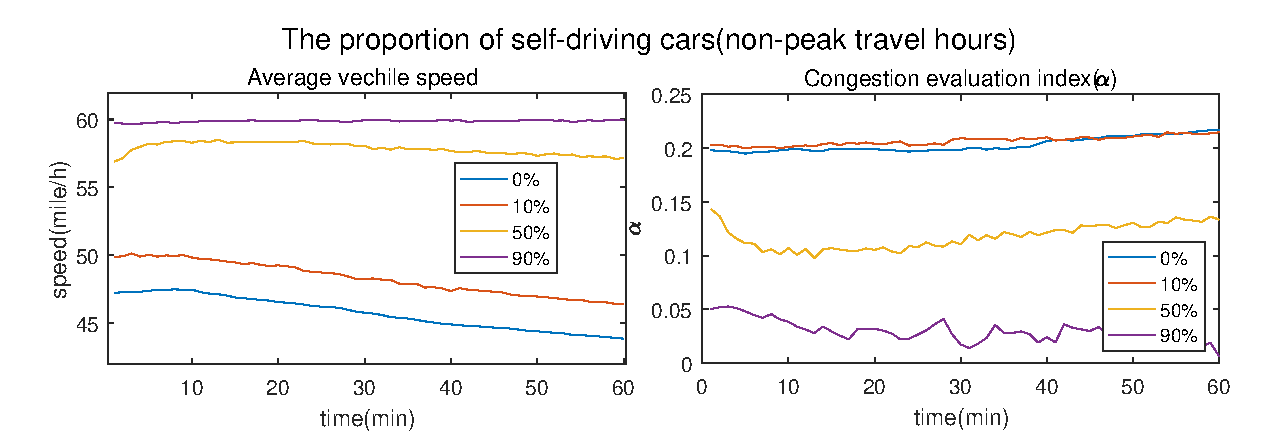
\includegraphics[height=5cm]{auto_all(5)-non-peak.eps}}
	\caption{Single step of the simulation}
\end{figure}
The figure below shows within the peak travel hours, the variations of $V_{i}$ and $\alpha_{i}$ within 60 minutes.\\
\begin{figure}[H]
	\centerline{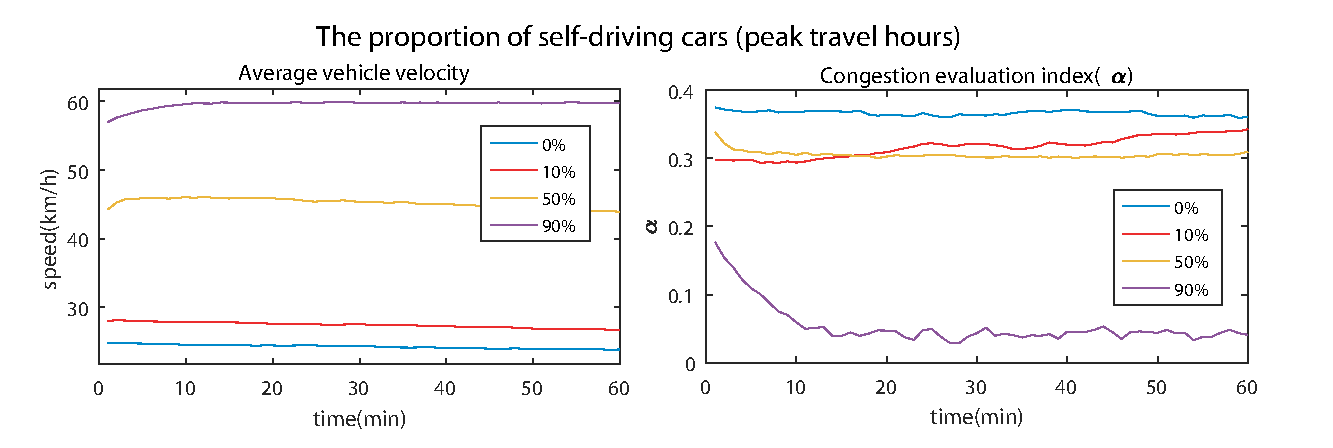
\includegraphics[height=5cm]{auto_all(5).eps}}
	\caption{Single step of the simulation}
\end{figure}
\indent The above figure shows in peak travel hours or non-peak hours, when the proportion of self-driving increases, the $V_{i}$ will increase and the $\alpha_{i}$ will decrease, which indicates the congestion will decrease with the proportion of self-driving increasing.\\
\indent And when proportion transfers from $50\%$ to $90\%$, the variation is remarkable. When the proportion reach $90\%$, the $V_{i}$ approaches the maximum allowed speed 60 miles per hour. So the operation efficiency of the road approaches maximum value. And there is little congestion occurred. \\


\subsection{The effects of cooperating systems}

\section{Model Validation}
\subsection{The Hydromechanics model in Traffic Flow}
	The related search use The Hydromechanics model to describe the process of traffic flow.\\
\indent\textbf{Aggregation wave}\\
\indent	A traffic flow wave moves from a low density to a high density state. For example, when the front road is very crowded, the front vehicles will speed down, and the rear car will speed down one after the other. The process is described as an aggregation wave that passes a signal from one vehicle to another vehicle.\\
\indent \textbf{Seperation wave}\\
\indent	A traffic flow wave moves from a high density to a low density state. For example, when the front road is very smooth, the front vehicles will speed up, and the rear car will speed up one after the other. The process is described as an aggregation wave that passes a signal from one vehicle to another vehicle.\\
\indent \textbf{Fluctuation of traffic flow}\\
\indent		Because of the existence of Aggregation wave and Seperation wave, some congested or smooth situation in the road will be passed by the wave rather than gather at a certain section of the road.\\
\indent \textbf{The speed of wave $W$}\\
\indent	The speed of Aggregation wave or Seperation wave.\\
\subsection{The calculation of $W$}
\indent The state of the traffic flow is described by the $K,v$.\\
\indent Suppose the initial state is $(K_{1}, v_{1})$, which means there are $K_{1}$ vehicles per meter, and the velocity of the vehicles is $v_{1}$. And the state of the next moment is $(K_{2}, v_{2})$. \\
\indent The $W$ is calculated by the equation:
\begin{equation}
	W=\frac{K_{1}v_{1}-K_{2}v_{2}}{K_{1}-K_{2}}
\end{equation}
\subsection{The discussion about the wave}
When $K_{2}>K_{1}$, it means the traffic flow wave moves from a low density to a high density state. So the wave is an aggregation wave. And if $ Q_{2}>Q_{1} $, the $W$ is a positive value, which means the direction of the aggregation wave is the same as that of the traffic flow. If $ Q_{1}<Q_{2} $, the $W$ is a negative value, which means the direction of the aggregation wave is opposite to that of the traffic flow. \\
\indent And we can discuss the situation when $K_{2}<K_{1}$The table below shows the different situation.\\
\begin{table}[H]
        \setlength{\abovecaptionskip}{0pt}
        \setlength{\belowcaptionskip}{0pt}
		\centering{Table 1: the direction and class of the wave in different situation}\\
        \begin{tabular}{p{2.7cm}<{\centering}|p{5.5cm}<{\centering}|p{5.5cm}<{\centering}|}
		\hline
		\rowcolor[gray]{0.9}\bf{}	&\bf{$K_{1}<K_{2}$}&\bf{$K_{1}>K_{2}$}	\\
		\hline
		$ Q_{1}<Q_{2} $	 & \makecell[{}{p{5.5cm}}]{\textbf{Direction}: Opposite to that of traffic flow;\\  \textbf{Class}: Aggregation wave  } &\makecell[{}{p{5.5cm}}]{\textbf{Direction}:The same as that of traffic flow;\\ \textbf{Class}: Seperation wave}\\
		\hline
		$Q_{1}>Q_{2} $  & \makecell[{}{p{5.5cm}}]{\textbf{Direction}: The same as that of traffic flow;\\  \textbf{Class}: Aggregation wave  }  
		&\makecell[{}{p{5.5cm}}]{\textbf{Direction}:Opposite to that of traffic flow;\\ \textbf{Class}: Seperation wave}
	\end{tabular}
\end{table}
\subsection{Use the Hydromechanics model to verify our CA model}
\indent In our simulation, we get the space distribution of vehicle density $K$ and traffic flow $Q$ in some time(15min, 30min, 45min, 60min from the beginning).\\
\indent The depth of the color in the figure represents the quantity of the vehicle density $K$ and traffic flow $Q$. And deeper the color is, larger the vehicle and the traffic flow is. The horizontal axis represents the distance from start of a section of the road.\\
\indent We pay attention to the congestion part of the section, and tag this part with a red circle.\\
\indent In the figure, we can find the $K_{red}$ and $Q_{red}$ is the largest in the road. So $K_{2}$ must be smaller than $K_{1}$, $Q_{2}$ must be smaller than $Q_{1}$. So according to the Table 1, there must be a Seperation wave of which the direction is to the end of the road  and an Aggregation wave of which the direction is to the start of the road.\\
\indent Therefore, the left part of the tagged part will be more crowded, the right part of the tagged part will be more smooth.\\
\indent And it means with the time goes, the crowded part(tagged) will shift to the left.\\
\indent So we observe the change of location of the tagged part.\\
\begin{figure}[H]
\centering
\subfigure[Spatial distribution of k,Q at 15 minutes]{
\begin{minipage}[b]{1\textwidth}
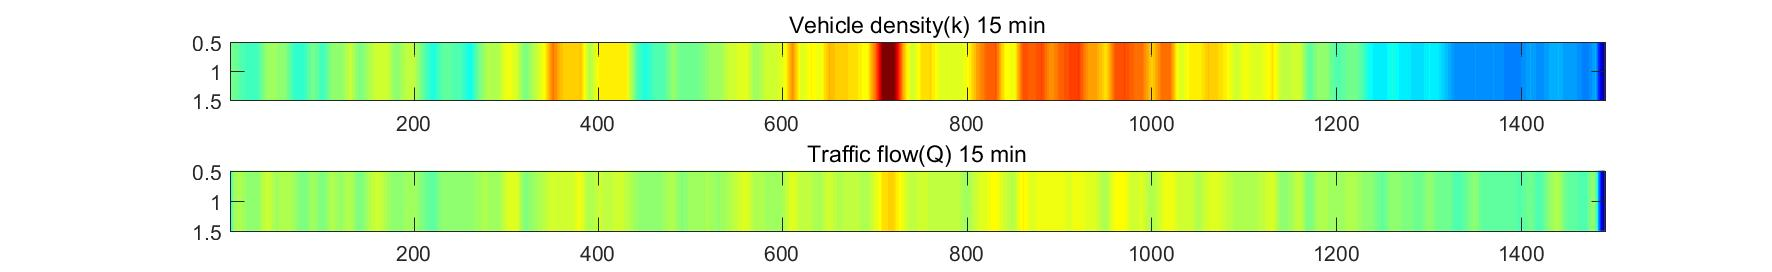
\includegraphics[width=1\textwidth]{fig15.jpg}
\end{minipage}
}
\subfigure[Spatial distribution of k,Q at 30 minutes]{
\begin{minipage}[b]{1\textwidth}
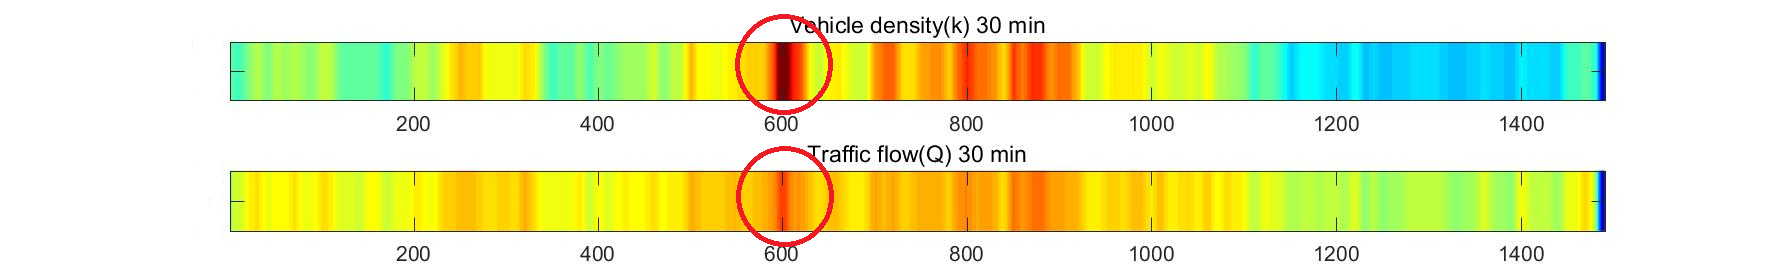
\includegraphics[width=1\textwidth]{fig30.png}
\end{minipage}
}
\subfigure[Spatial distribution of k,Q at 45 minutes]{
\begin{minipage}[b]{1\textwidth}
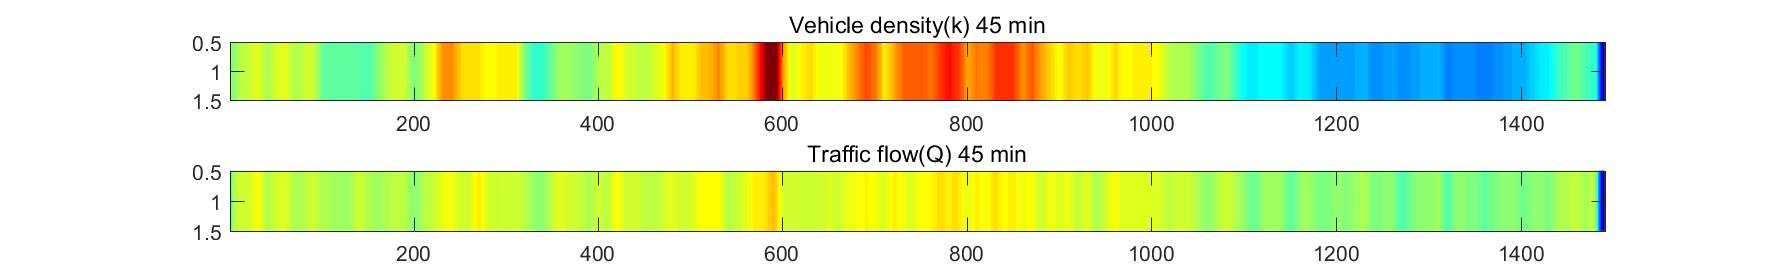
\includegraphics[width=1\textwidth]{fig45.jpg}
\end{minipage}
}
\subfigure[Spatial distribution of k,Q at 60 minutes]{
\begin{minipage}[b]{1\textwidth}
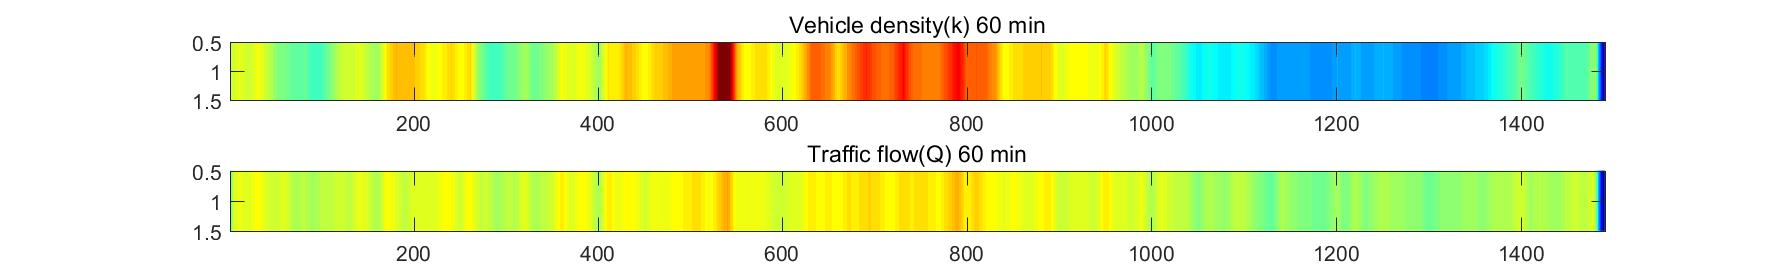
\includegraphics[width=1\textwidth]{fig60.jpg}
\end{minipage}
}
 \caption{Spatial distribution of k,Q at different moments} \label{fig:1}
\end{figure}
\indent From the above figure, we find that actual change of the location of the tagged part is consistent with the classic Hydromechanics model in traffic flow. \\
\indent Therefore, our model and simulation are reliable.


\section{Sensitivity Analysis}
\subsection{Initial velocity of simulation}

\subsection{Change of HT}

\subsection{Change of Peak time}

\section{Strengths and Weaknesses}

\section{A letter to the Governor's office}
As the population grows and the number of private cars has increasingly becoming large, the drives will experience long delays when there is congestion in the road. However, it costs a lot to build a new road, and the fundamental problem still can not be solved.\\
\indent With the progress of science and technology, the technology of self-driving has become more and more mature. We can consider increasing the proportion of self-driving to reduce road congestion.
In our paper, our model discuss the influence on the traffic flow from different proportion of self-driving in peak travel hours and non-peak travel hours. Because the self-driving is controlled by sensors and computers, they will spend little time to make a corresponding reaction. Therefore, the Time Headway between two self-drivings can be very short, and the distance between them can be close.\\ \indent In our model, we can find the larger the proportion of the self-driving is, the more smooth the road is, and the less congestion there is. \\
\indent At the same time, the self-driving vehicles can arrive at the destination automatically. The driver will not be banned from drinking, sleeping when the vehicles travel on the road.
We make some suggestion for some policy changes:\\
\indent 1.Give allowance or impose less taxes when citizens purchase self-driving.\\
\indent 2.More road toll is paid when the manual-driving passes the toll-gate.\\
\indent 3.According to the proportion of self-driving, use a few lanes as a special driveway for self-driving vehicles.\\
\indent Therefore, use a large proportion of self-driving can reduce the congestion effectively. If our suggestion is adopted, the transportation in Washington will be very smooth, and citizens will experience a comfortable and time-saving travel. 


\section{References}
\begin{thebibliography}{99}
\bibitem{TF1}CREMER M, LUDWIG J. A Fast Simulation Model for Traffic Flow on the Basis of Boolean Operations [J ] . Mathematics and Computers in Simulation, 1986,28(4): 297-303.
\bibitem{TF2}Ding Jian-xun, WANG Ni-shang, SHI Qin. A Two-dimensional BML Model of Traffic Flow Considering Overpass Configuration [ J ]. Journal of Transportation Systems Engineering and Information Technology, 2011,11(6): 98-103
\bibitem{ca1}Nagel K, Schreckenberg M. A cellular automaton model for freeway traffic[ J ].J Phys I : France, 1992,12(2):2221-2229
\bibitem{ca2}Takayasu M,Takayasu H.I/f  noise in a traffic model[ j ]. Fractal -complex Geometry Patterns \& Scaling in Nature \& Society,1996,29(12):3119-3127(9)
\bibitem{ca3}Barlovic R, Santen L, Scnadschneider A. Metas-table states in cellular automate[ J ]. the European Physical Joural B,1998(3): 793-800
\bibitem{ca4}SHI Jun-qing, CHENG Lin, long Jian-cheng, et al.A New Cellular Automaton Model for Urban Two-way Road Networks [ J ]. Computational Intelligence and Neuroscience, 2014,2014;685047
\bibitem{TH}Zhang G, Wang Y, Wei H, et al. Examining headway distribution models with urban freeway loop event data[J]. Transportation Research Record Journal of the Transportation Research Board, 2007, 1999(1):141-149.
\end{thebibliography}



\end{document}